\documentclass[a4paper,11pt]{ltjsarticle}
\usepackage{luatexja}
\usepackage{amsmath,amssymb,mathtools}
\usepackage{bm}
\usepackage{tikz}
\usepackage{tikz-cd}
\usepackage{enumitem}
\usepackage{geometry}
\usepackage[hidelinks]{hyperref}  % しおり／相互参照を有効化
\geometry{margin=25mm}

\usetikzlibrary{arrows.meta,calc,decorations.pathmorphing}

\title{離散フィルトレーションと構造塔の入門\\\smallskip
{\large--- Gemini モジュールの学部生向け解説 ---}}
\author{CODEX (OpenAI)\\Lean ファイル生成: CODEX (OpenAI)}
\date{2025年11月5日}

\begin{document}

\maketitle

\begin{abstract}
本資料は、Lean ファイル \texttt{MyProjects/ST/Gemini.lean} で実装された
\emph{StructureTowerWithMin} の離散確率論的解釈を、学部初期を想定した読者向けに解説する。
自然数上のフィルトレーションをどのように構造塔として表現するか、最小層関数
\(\mathrm{minLayer}\) が停止時刻の条件を満たす理由、そして射の条件が
「非先見的」な写像を強制する様子を図式付きで説明する。
\end{abstract}

\tableofcontents

\section{序論}

ボルバキの『数学原論』では、数学的対象を「集合と構造」の言葉で統一的に扱う。
構造塔（Structure Tower）は、この精神をそのままに受け継ぎ、
集合 \(X\) の上に指数集合 \(I\) で整列した「層」
\(\bigl(X_i\bigr)_{i\in I}\) を備え、各点 \(x\in X\) が初めて出現する最小の層
\(\mathrm{minLayer}(x)\) を持つデータである。

Lean ファイル \texttt{Gemini.lean} では、この構造塔を離散時間の確率論に応用し、
自然数上の最も単純なフィルトレーションを復元した。
本ノートではその内容を噛み砕き、直感と背景を補う。

\section{構造塔の基本}

\subsection{定義の要点}

構造塔 \(\mathcal{T} = (X, I, \leq, (X_i)_{i\in I}, \mathrm{minLayer})\) は次を満たす。
\begin{enumerate}[label=(\arabic*)]
  \item 任意の \(x\in X\) に対し、ある層 \(X_i\) が \(x\) を含む（被覆性）。
  \item 指数の順序 \(i\leq j\) に対し \(X_i\subseteq X_j\)（単調性）。
  \item 各 \(x\) は最小の層 \(\mathrm{minLayer}(x)\) に属し、他の層はそれ以上の指数である。
\end{enumerate}

Lean ではこれらの条件が構造体 \verb|StructureTowerWithMin| にまとめられている。
\texttt{Gemini.lean} では、自然数版
\[
  \mathrm{FiltrationTowerNat} : X = \mathbb{N},\quad I = \mathbb{N},\quad
  X_n = \{k\in\mathbb{N} \mid k\leq n\},\quad
  \mathrm{minLayer}(k)=k
\]
をそのまま実装し、既存の \verb|natTowerMin| と同一視している。

\subsection{停止時刻としての \texorpdfstring{\(\mathrm{minLayer}\)}{minLayer}}

離散フィルトレーション \((\mathcal{F}_n)_{n\in\mathbb{N}}\) において、
停止時刻 \(\tau\) とは \(\{\omega \mid \tau(\omega)\leq n\}\in\mathcal{F}_n\) を満たす写像である。
Lean 定理
\[
  \mathrm{minLayer\_is\_stopping\_time}
\]
は構造塔の公理のみを用いて
\(\{x \mid \mathrm{minLayer}(x)\leq i\}\subseteq X_i\) を示し、
この条件が一般の塔でも自動的に成り立つことを保証する。
確率論的には「要素が初めて観測される時刻は、ちょうどその時刻の情報に含まれる」という自然な事実を形式化したものである。

\section{射と非先見性}

\subsection{射の条件}

塔の射 \(\varphi : \mathcal{T}\to\mathcal{T}'\) は基礎集合写像
\(\varphi_{\mathrm{map}}\) と指数写像 \(\varphi_{\mathrm{index}}\) の組であり、
層構造と最小層を保つ必要がある。
特に重要なのが最小層の保存
\[
  \mathrm{minLayer}'\bigl(\varphi_{\mathrm{map}}(x)\bigr)
    = \varphi_{\mathrm{index}}\bigl(\mathrm{minLayer}(x)\bigr).
\]
これは「情報が早まらない・遅れない」ことを表す。

\subsection{\texorpdfstring{\(\mathrm{succ}\)}{succ} が射にならない理由}

\texttt{Gemini.lean} の定理
\[
  \mathrm{succ\_not\_hom\_with\_id\_indexMap}
\]
は、指数写像が恒等であると仮定すると \(\mathrm{succ}\colon n\mapsto n+1\) は射になり得ないことを示す。
図式的には次のように理解できる（図\ref{fig:succ}）。

\begin{figure}[htbp]
  \centering
  \begin{tikzcd}[row sep=huge, column sep=huge]
    x \arrow[d, dashed, "\varphi_{\mathrm{map}}=\mathrm{succ}"'] \arrow[r, hook, "\mathrm{minLayer}(x)=x"] &
      X_x \arrow[d, hook, "\subseteq"] \\
    x+1 \arrow[r, hook, "\mathrm{minLayer}(x+1)=x+1"'] &
      X_{x+1}
  \end{tikzcd}
  \caption{\(\mathrm{indexMap}=\mathrm{id}\) を保ったまま \(\mathrm{succ}\) を許すと、
  左上の要素が右下へ写るため、\(\mathrm{minLayer}\) が保存されない。}
  \label{fig:succ}
\end{figure}

例えば \(x=0\) を取ると、\(\mathrm{minLayer}(0)=0\) である一方、
\(\mathrm{minLayer}(\mathrm{succ}(0))=1\) となり、指数側が恒等である限り一致しない。
従って、射は必然的に恒等写像になる。これは「未来の情報は見えない」という
停止時刻の直感と整合的である。

\section{直積と σ-代数}

\subsection{塔の直積}

Lean の定義
\[
  \mathrm{FiltrationTowerNatProd} = \mathrm{prod}\bigl(\mathrm{FiltrationTowerNat},
  \mathrm{FiltrationTowerNat}\bigr)
\]
は、基礎集合を \(\mathbb{N}\times\mathbb{N}\)、指数集合を \(\mathbb{N}\times\mathbb{N}\) とし、
層を直積 \(X_{\langle i,j\rangle} = X_i\times X_j\) によって与える。
\texttt{layer\_nat\_prod} ではこれが明示的に
\[
  X_{\langle i,j\rangle} = \{(a,b)\in\mathbb{N}\times\mathbb{N}\mid
  a\leq i,\; b\leq j\}
\]
であることを確認している。

\subsection{σ-代数との違い}

確率論でいうフィルトレーションの直積は、集合の単純直積ではなく、
直積集合によって生成される最小の σ-代数である。
図\ref{fig:rectangle} のように、構造塔の層は長方形（有限の情報）で止まっているのに対し、
σ-代数は可算和や補集合を閉じる必要がある。

\begin{figure}[htbp]
  \centering
  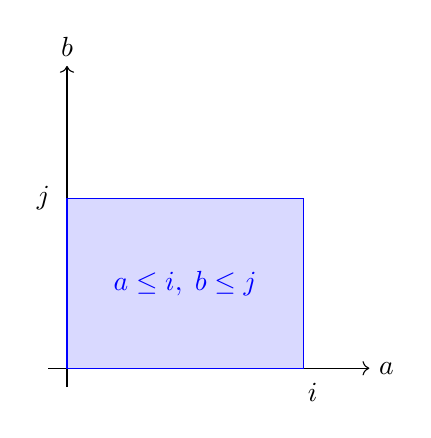
\begin{tikzpicture}[scale=1.2]
    \draw[->] (-0.2,0) -- (3.2,0) node[right] {$a$};
    \draw[->] (0,-0.2) -- (0,3.2) node[above] {$b$};
    \draw[fill=blue!15, draw=blue] (0,0) rectangle (2.5,1.8);
    \draw[dashed, color=blue] (2.5,0) -- (2.5,1.8);
    \draw[dashed, color=blue] (0,1.8) -- (2.5,1.8);
    \node[blue] at (1.25,0.9) {$a\leq i,\; b\leq j$};
    \node at (2.6,-0.25) {$i$};
    \node at (-0.25,1.8) {$j$};
  \end{tikzpicture}
  \caption{構造塔の層は長方形集合のレベルに留まる。σ-代数を得るには、この図を生成する可算操作を追加で許す必要がある。}
  \label{fig:rectangle}
\end{figure}

そのため、構造塔の直積は「生成系」を与え、σ-代数の直積はその上位概念である。
この差異を理解しておくと、測度論的議論に発展する際の混乱を避けられる。

\section{まとめと今後の展望}

\begin{itemize}
  \item \(\mathrm{minLayer}\) は停止時刻の条件を自動的に満たし、構造塔と確率論の橋渡しをする。
  \item 射は最小層を厳密に保存するため、`Nat.succ` のような「時間を先送りする」写像は許されない。
  \item 直積は σ-代数の直積と異なり、まずは長方形集合の階層を与えるものである。
\end{itemize}

連続時間版フィルトレーションや、σ-代数を直接レベルとして持つ拡張を考えると、
構造塔の枠組みがさらに豊かに応用できる。Lean ファイル \texttt{Gemini.lean} は
その第一歩として、離散確率論の基本例を形式的に位置づけている。

\end{document}
